\nnarticleheader{Lagrange Points: Solving for Gravitational Parking Spaces}{Alexander Greer, Haverford '20}
\noindent
\textbf{Introduction}

Picture your middle school science class: you are working through a unit on forces and your teacher is making an analogy for gravity. He has set up a big rubber sheet, at the center of which he has placed a heavy steel ball. The ball weighs down the sheet to form a sort of funnel. He then places a marble at the edge of the sheet and asks you what might happen if he lets go. You, being a well-informed science student, suggest that the marble will roll around and around the funnel created by the ball in a sort of orbit. Your teacher releases the marble and it follows exactly the path you expected. Then, your teacher recovers the small marble, adds another steel ball before asking another question: what will happen to the path of the marble if it conserves its angular velocity given that the entire sheet is in a rotating reference frame?

This, obviously far beyond the scope of a middle school science class, turns out to be a very difficult problem to solve. It is called the \textit{three-body problem} and has challenged physicists and mathematicians since Newton developed his laws of motion. Through centuries of study, we have found that there is, in fact, no closed-form solution to the motion of three bodies. That is, subsequent movement of the bodies cannot be predicted without equations of infinite magnitude.

Applications of the three-body problem are not entirely hopeless, however. Systems like the Earth, Moon, and Sun indicate that there has to be some quantifiable pattern in behavior. One method is to solve a \textit{restricted} three-body problem, defined by one body of negligible mass under the influence of two more massive bodies. In 1772, Franco-Italian mathematician and astronomer Joseph-Louis Lagrange discovered a series of points at which such a body could maintain a stable position relative to the movement of the other two. A small enough object would be caught in a series of opposing gravitational forces that all cancel out. These five “Lagrange Points” are extremely useful for astrophysicists to “park” objects in space. Things like satellites can remain in a stable position without falling into orbit around the two massive bodies while requiring minimal energy to do so.
\newline\newline
\textbf{Explanation}

Three of these Lagrange points (notated $L_1,$ $L_2,$ and $L_3$) exist collinearly on the axis defined by the two massive bodies. They are “nominally unstable,” meaning they require some energy input in order for a third body to maintain position over long periods of time. The other two points ($L_4$ and $L_5$) are at the corners of equilateral triangles in the plane of orbit whose common base is the line between the centers of the two massive bodies. In the solar system, many natural satellites can be found around the $L_4$ and $L_5$ points of various planets, as they are naturally stable and provide undisturbed equilibrium (Figure 1). 

\begin{figure}[h]
  \begin{center}
    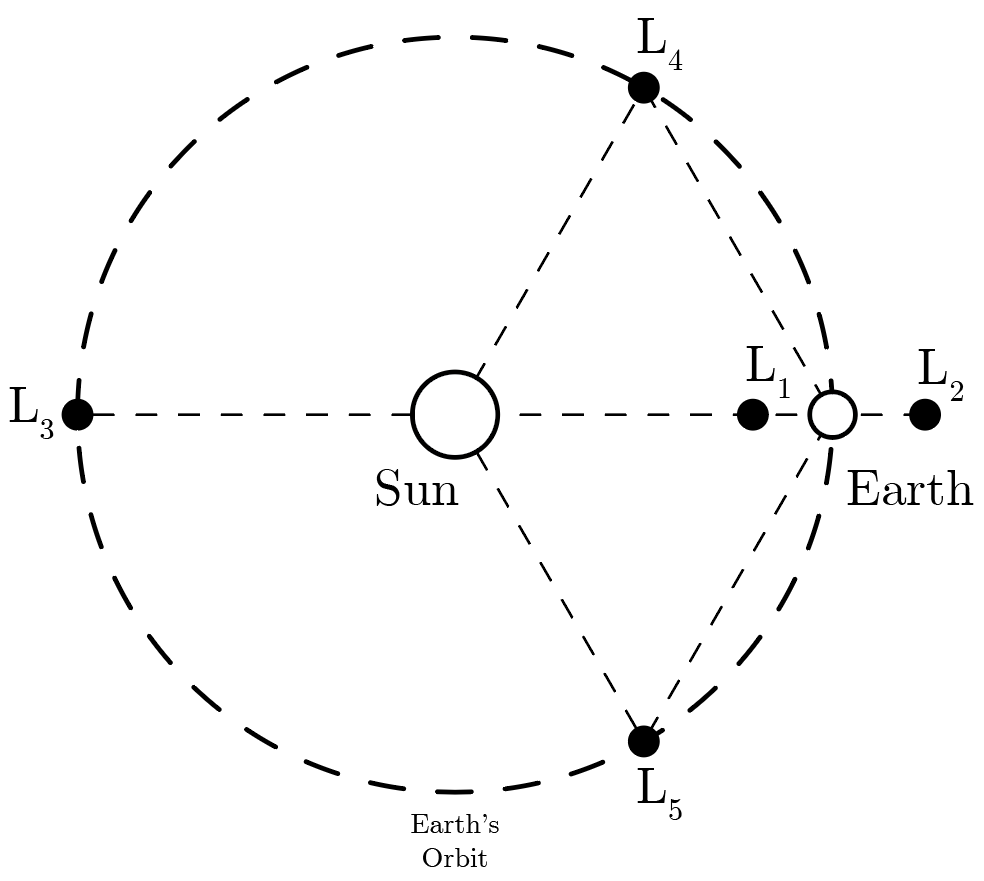
\includegraphics[scale=.6]{greer_lagrange_fig_1}
  \end{center}
  \caption{The five Lagrange points.}
  \label{fig:1}
\end{figure}

The derivation for these points is based on Newton’s Law of Gravitation, which describes the force of gravity between two objects based on their masses and distance from one another: \[F_g = G\frac{m_1m_2}{r^2}\]

$m_1$ and $m_2$ are the masses of both objects in kilograms, $r$ is the distance between the two in meters, and $G$ is the gravitational constant equal to $6.674\times{10^{-11}} \frac{m^3}{kg\cdot{}s^2}$.
\newline\newline
\textbf{Derivation}

Unfortunately, because of the physical nature of our universe, there is no simple law of gravitation for three distinct bodies. That would make this problem a whole lot easier. To find Lagrange points in a restricted three-body problem, we can certainly apply the Law of Gravitation, but we’ll end up approximating the points’ positions. For the use cases on Earth, however, these approximations are more than adequate. 

We can observe the figure below (Figure 2) to see how each of the masses act on each other. 

\begin{figure}[h]
  \begin{center}
    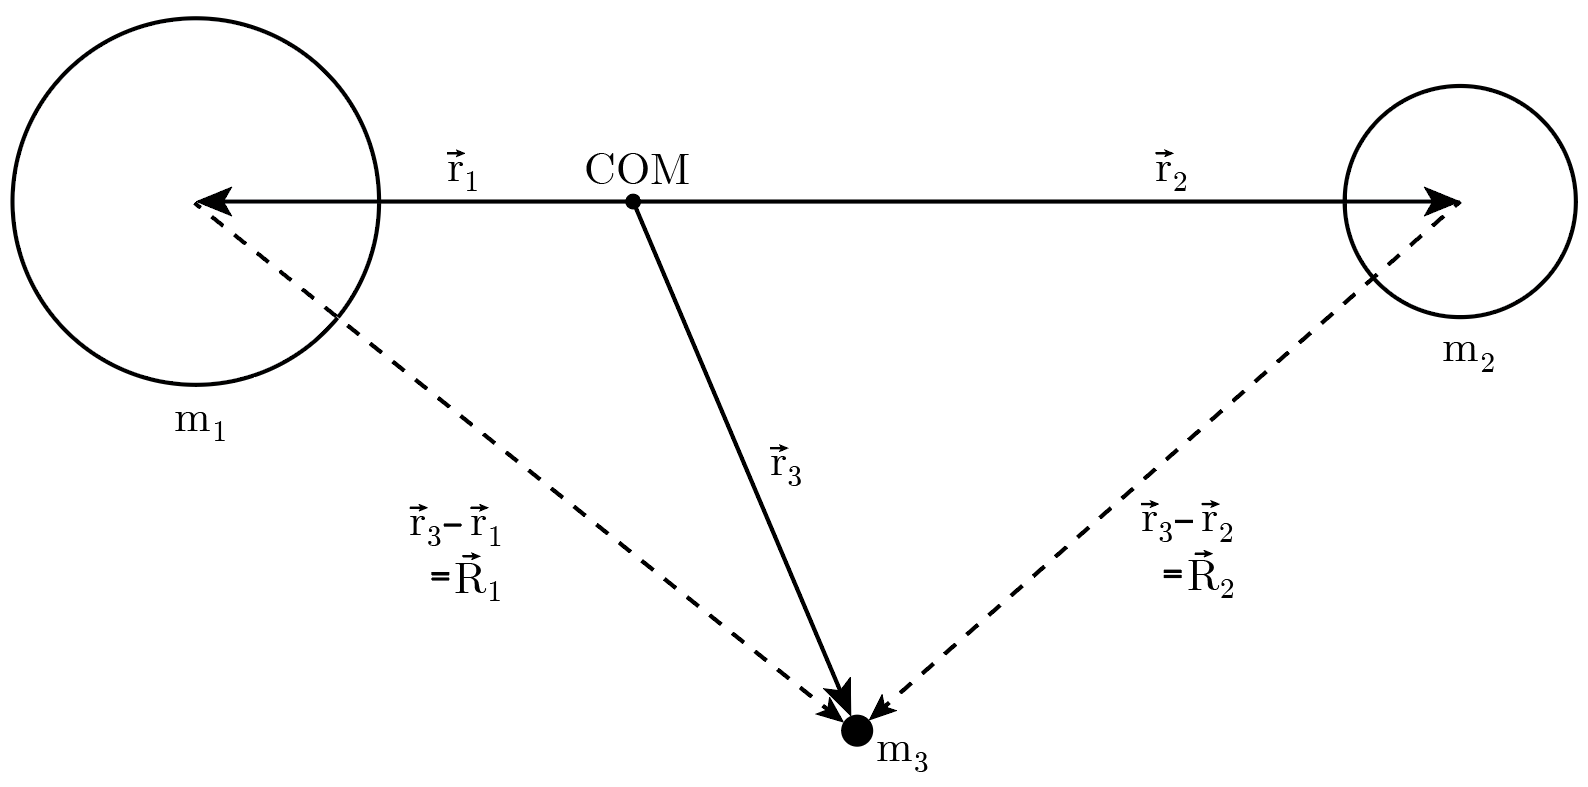
\includegraphics[scale=.6]{greer_lagrange_fig_2}
  \end{center}
  \caption{Gravitational forces in a restricted three body problem.}
  \label{fig:2}
\end{figure}

$m_1$ and $m_2$ are the large masses of this system (for example, the Sun and the Earth). $m_3$ is the third mass of negligible magnitude. We use position vector representations of the distances between objects. These are relative to the system’s center of mass (COM). $\vec{r_1}$, $\vec{r_2}$, and $\vec{r_3}$ represent the positions of $m_1$, $m_2$, and $m_3$, respectively. We can denote the direction of the forces acting on m3 by subtracting each other mass’ position vector. The force of $m_1$ on $m_3$ is in the direction of $\vec{r_3}-\vec{r_1}$, which we can denote as $\vec{R_1}$. Thus the force of $m_2$ on $m_3$ follows $\vec{r_2}-\vec{r_1}$, denoted as $\vec{R_2}$

The total force on $m_3$ equals the sum of the forces on it by both $m_1$ and $m_2$, as below: 
\[F_T=F_{1\rightarrow3} + F_{2\rightarrow3}\]

Plugging in our position vectors, we arrive at the below equation:
\[F_T=G\frac{m_1m_3}{|\vec{R_1}|^2}\hat{R_1}+G\frac{m_2m_3}{|\vec{R_2}|^2}\hat{R_2}\]
which can be simplified as:
\[F_T=m_3G(\frac{m_1}{|\vec{R_1}|^2}\hat{R_1}+\frac{m_2}{|\vec{R_2}|^2}\hat{R_2})\]

$\hat{R_1}$ and $\hat{R_2}$ denote unit vectors in the directions of the present forces, equal to $\frac{\vec{r_3}-\vec{r_1}}{|\vec{r_3}-\vec{r_1}|}$ and $\frac{\vec{r_3}-\vec{r_2}}{|\vec{r_3}-\vec{r_2}|}$, or $\frac{\vec{R_1}}{|\vec{R_1}|}$ and $\frac{\vec{R_2}}{|\vec{R_2}|}$, respectively. 

The next aspect that plays into our derivation is the angular frequency ($\Omega$) of the entire system. In our sun-Earth example, there are pseudo-forces acting on the third mass based on the orbital rotation of the entire system. This is described by Kepler’s Third Law of Planetary Motion:
\[\frac{r^3}{T^2}=\frac{G(m_1+m_2)}{4\pi^2}\]
where $r$ is the radius of the orbit and $T$ is the orbital period. Angular frequency is equal to $\Omega=\frac{v}{r}$, and the orbital period is equal to $T=\frac{2\pi r}{v}$. Knowing this, we can plug in and do some algebraic shuffling to get:
\[\Omega^2r^3=G(m_1+m_2)\]
which can then be used to solve for angular frequency:
\[\Omega=\sqrt{\frac{G(m_1+m_2)}{r^3}}\]

The final piece to our puzzle is to quantify the pseudo-forces acting on our system described previously. A rotating reference frame implies the addition of both the Coriolis force and the centrifugal force. The Coriolis force (known commonly as the Coriolis effect) is responsible for things like cyclone formation as the Earth spins, and you may remember the centrifugal force from your middle school science teacher swinging a bucket of water above their head. We account for these pseudo-forces by subtracting out their values from the force equation derived above:
\[F_{\Omega}=F_T-2m(\Omega\times\frac{dr}{dt})-m\Omega\times(\Omega\times r)\]
where the Coriolis force is $-2m(\Omega\times\frac{dr}{dt})$ and the centrifugal force is $-m\Omega\times(\Omega\times r)$.

Performing a bit more inference using equations involving generalized potential energy (see the sources for an in-depth explanation), we can plot our result using a computer program on a 3D contour map (Figure 3).

\begin{figure}[h]
  \begin{center}
    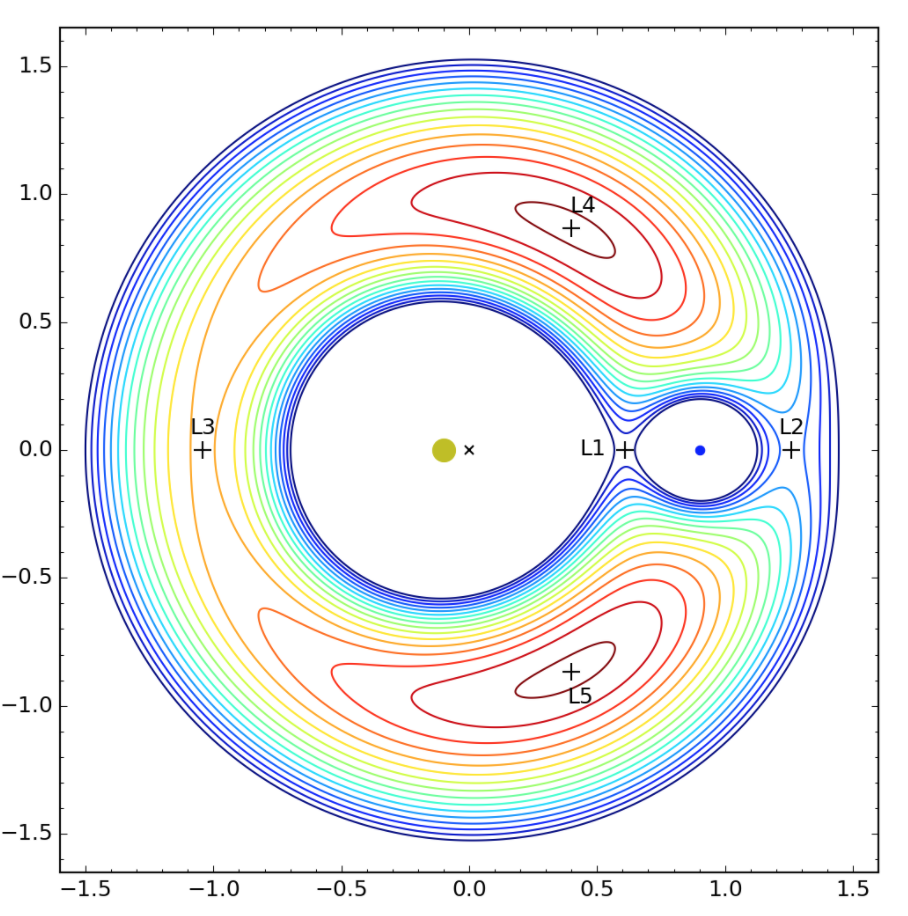
\includegraphics[scale=.7]{greer_lagrange_fig_3}
  \end{center}
  \caption{A contour plot of gravitational energy revealing the locations of the five Lagrange points.}
  \label{fig:3}
\end{figure}

The extrema of this graph display places where the various gravitational potentials cancel out: the Lagrange points. In the sun-Earth system, points $L_1$ and $L_2$ are about 1.5 million kilometers on either side of the Earth. $L_3$ is approximately opposite Earth at its orbital distance of about 150 million kilometers. $L_4$ and $L_5$ are each 1.5 million kilometers away from Earth at 60-degree angles.
\newline\newline
\textbf{Conclusion}

The math to get here may have been a bit complicated, and there were certainly some aspects left out for clarity, but at its essence, this derivation demonstrates the simplistic beauty of the laws of our universe. Something as simple as two objects floating around each other can produce complex curves and dips in spacetime where asteroids, satellites, and telescopes can float without worry. Maybe one day in the future humanity will escape the bonds of Earth and rest comfortably in a gravitational valley created by its home planet, looking out at the unknown wonders hidden amongst the stars. 
\newline\newline
\textbf{Sources}

For a full derivation of each individual point using an approximation technique called perturbation theory, check out the following paper by Dennis Westra of the University of Vienna: 
\newline\url{https://www.mat.univie.ac.at/~westra/lagrangepoints.pdf}

Also check out these notes created by NASA outlining the steps used in this article, as well as some more interesting calculus relating to the problem:
\newline\url{https://map.gsfc.nasa.gov/ContentMedia/lagrange.pdf}

Image source: 
\newline\url{https://leancrew.com/all-this/2016/08/lagrange-points-redux/}